\documentclass[10pt]{article}
\usepackage{fullpage}
\usepackage{graphicx}
\usepackage{amssymb}
\usepackage{qtree}
\usepackage{rotating}
\newcommand{\tab}{\hspace*{2em}}
\newcommand{\tabb}{\hspace*{4em}}
\newcommand{\tabbb}{\hspace*{6em}}
\newcommand{\tabbbb}{\hspace*{8em}}
\newcommand{\tabbbbb}{\hspace*{10em}}
\newcommand{\norm}[1]{\left|\left|#1\right|\right|}
\setlength{\parindent}{0in} 
\begin{document}
	\begin{flushright}
	Lindsey Bieda and Joe Frambach\\
	Dynamic Programming Problems\\
	10.19.2011
	\end{flushright}
		7. Show that if one of the following three problems has a polynomial time algorithm then they all do.
		\begin{itemize}
		\item The input is two undirected graphs $G$ and $H$. The problem is to determine if the graphs are
		isomorphic. (referred to as ISOGRAPH)
		\item The input is two directed graphs $G$ and $H$. The problem is to determine if the graphs are
		isomorphic. (referred to as ISODIGRAPH)
		\item The input is two undirected graphs $G$ and $H$, and an integer $k$. The problem is to determine if
			  the graphs are isomorphic and all the vertices in each graph have degree $k$. (referred to as KISOGRAPH)
		\end{itemize}
		Intuitively, two graphs are isomorphic if on can name/label the vertices so that the graphs are identical.
		More formally, two undirected graphs $G$ and $H$ are isomorphic if there is a bijection $f$ from the vertices
		of $G$ to the vertices of $H$ such that $(v, w)$ is an edge in $G$ if and only if $(f (v), f (w))$ is an edge in $G$.
		More formally, two directed graphs $G$ and $H$ are isomorphic if there is a bijection $f$ from the vertices
		of $G$ to the vertices of $H$ such that $(v, w)$ is a directed edge in $G$ if and only if $(f (v), f (w))$ is a directed
		edge in $G$. The degree of a vertex is the number of edges incident to that vertex.
		\\
		\\
		KISOGRAPH $\leq$ ISOGRAPH\\
		\\
		program KISOGRAPH:\\
		\tab Read $G,H,k$.\\
		\tab $g$ = \# vertices in $G$\\
		\tab $h$ = \# vertices in $H$\\
		\tab If $g \neq h$ return 0\\
		\tab For all vertices n = 1 to g:\\
		\tabb count = 0\\
		\tabb For all vertices m = 1 to g, m $\neq$ n:\\
		\tabbb If edge (n,m) exists in G:\\
		\tabbbb count = count + 1\\
		\tabb if count $\neq$ $k$:\\
		\tabbb Return 0.\\
		\tab For all vertices n = 1 to g:\\
		\tabb count = 0\\
		\tabb For all vertices m = 1 to g, m $\neq$ n:\\
		\tabbb If edge (n,m) exists in H:\\
		\tabbbb count = count + 1\\
		\tabb if count $\neq$ $k$:\\
		\tabbb Return 0.\\
		\tab Return ISOGRAPH(G,H).\\
		\\
		Just check the degree of the vertices in $G$ and $H$ and then if that is valid return the result of ISOGRAPH. The degree checking will
		take $O(n^2)$ time.\\
		\\
		\\
		ISOGRAPH $\leq$ ISODIGRAPH\\
		\\
		program ISOGRAPH:\\
		\tab Read $G$, $H$\\
		\tab Create $G^\prime$ and $H^\prime$ by replacing every edge with two directed edges in both directions ($O(n^2)$)\\
		\tab Return ISODIGRAPH($G^\prime$, $H^\prime$).\\
		\\
		Since the new graphs generated from the input contain every edge going in opposite directions they are equivalent
		to the undirected graphs, since now the direction of the edge does not matter.\\
		\\
		\\
		ISODIGRAPH $\leq$ ISOGRAPH\\
		\\
		Read $G$, $H$\\
		Replace every directed edge with three additional vertices, forming a directional ``gate" using undirected edges, as in the following figure.\\
		\begin{figure}[h]
			\centering
			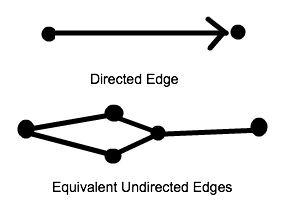
\includegraphics[width=300px]{21digraph.png}
		\end{figure}
		This is an O($n^2$) operation for $n$ the number of vertices.\\
		Return ISOGRAPH($G$,$H$).\\
		\\
		\newpage
		9. The input to the Hamiltonian Cycle Problem is an undirected graph $G$. The problem is to find a
		Hamiltonian cycle, if one exists. A Hamiltonian cycle is a simple cycle that spans $G$. Show that the
		Hamiltonian cycle problem is self reducible. That it, show that if there is a polynomial time algorithm
		that determines whether a graph has a Hamiltonian cycle, then there is a polynomial time algorithm
		to find Hamiltonian cycles.
		\\
		\\
		Hamiltonian Cycle Optimization $\leq$ Hamiltonian Cycle Decision.\\
		\\
		program hamiltonian cycle optimization:\\
		\tab read $G$\\
		\tab If $G$ has a hamiltonian cycle: \emph{call to hamiltonian cycle}\\ 
		\tabb for each node, $n$ in $G$:\\
		\tabbb $G^\prime = G - n$\\
		\tabbb If $G^\prime$ has a hamiltonian cycle:\\
		\tabbbb $G = G^\prime$\\
		\tab output $G$
		\\
		\newpage
		13. Show that the following problem is $NP$-hard:\\
		INPUT: A graph $G$. Let $n$ be the number of vertices in $G$.\\
		OUTPUT: 1 if $G$ contains a simple cycle with $\sqrt{n}$ edges, and 0 otherwise.\\
		Use the fact the the following problem is $NP$-hard:\\
		INPUT: A graph $G$.\\
		OUTPUT: 1 if $G$ contains a simple cycle that spans $G$, and 0 otherwise.\\
		Note that a cycle is simple if it doesn’t visit any vertex more than once. A cycle spans $G$ if every
		vertex is included in the cycle.\\
		\\
		Simple Cycle (SC) $\leq$ Simple Cycle Square Root (SCSR)\\
		\\
		program SC:\\
		\tab read $G$\\
		\tab $n$ = number verticies in $G$\\
		\tab $H$ = $n$ disjoint copies of $G$\\
		\tab output SCSR($H$)\\
		\\
		We've created a graph, $H$, with $n^2$ vertices. Since the copies of $G$ are disjoint the only case in which a simple cycle of 
		length $\sqrt{n}$ will appear is when there is a simple cycle spanning $G$.
\end{document}
